\documentclass[11pt,a4paper]{article}

% Modèle de rapport de stage et conseils de rédaction, mise en page...
% L. Bellon, avril 2010

% définition des marges du document
\setlength{\topmargin}{0cm}
\setlength{\headheight}{0.4cm}
\setlength{\headsep}{0.8cm}
\setlength{\footskip}{1cm}
\setlength{\textwidth}{17cm}
\setlength{\textheight}{25cm}
\setlength{\voffset}{-1.5cm}
\setlength{\hoffset}{-0.5cm}
\setlength{\oddsidemargin}{0cm}
\setlength{\evensidemargin}{0cm}


% quelques package utiles
%\usepackage{graphicx} % inclusion des figures
\usepackage{soul}
\usepackage{amsmath} % collection de symboles mathématiques
\usepackage{amssymb} % collection de symboles mathématiques
\usepackage[utf8]{inputenc}       % utilisation directe des caractères accentués sur pc
\usepackage[T1]{fontenc} % codage moderne des caractères sous Latex

\usepackage[francais]{babel}           % style français

\usepackage{tabularx} % gestion avancée des tableaux

\usepackage{psfrag} % remplacement du texte d'une figure ps par du texte latex
%\usepackage{sistyle} % mise en forme des unités

\usepackage{breqn}
\usepackage{eurosym} % symbole €
\usepackage{epstopdf} 
\def\€{\euro{}}

\usepackage[demo]{graphicx}
%\usepackage{caption}
\usepackage{subcaption}

\usepackage{color} % gestion de différentes couleurs

\definecolor{linkcolor}{rgb}{0,0,0.6} % définition de la couleur des liens pdf
\usepackage[ pdftex,colorlinks=true,
pdfstartview=FitV,
linkcolor= linkcolor,
citecolor= linkcolor,
urlcolor= linkcolor,
hyperindex=true,
hyperfigures=false]
{hyperref} % fichiers pdf 'intelligents', avec des liens entre les références, etc.

\usepackage{fancyhdr} % entêtes et pieds de pages personnalisés

% définition de l'entête et du pied de page
\pagestyle{fancy}
\fancyhead[L]{\scriptsize \textsc{Stage M2}}
\fancyhead[R]{\scriptsize \textsc{Clément Henin}}
\fancyfoot[C]{ \thepage}

% commande d'annulation du correcteur typographique du package [francais]{babel} qui force l'espace avant ':' (parfois utile pour la bibliographie)
\makeatletter
\@ifpackageloaded{babel}%
        {\newcommand{\nospace}[1]{{\NoAutoSpaceBeforeFDP{}#1}}}%  % !! double {{}} pour cantonner l'effet à l'argument #1 !!
        {\newcommand{\nospace}[1]{#1}}
\makeatother

% commande de déplacement d'un objet
\newcommand{\drawat}[3]{\makebox[0pt][l]{\raisebox{#2}{\hspace*{#1}#3}}}

\begin{document}

\title{Une interrogation sur la validité de l'utilisation de \og dummy variables \fg~pour prédire la croissance dans l'étude \textit{A Reassessment of the Relationship between Inequality and Growth} (2000)}

\maketitle

Le consensus sur les liens entre la croissance et les inégalités de revenus semble difficile à obtenir parmi les spécialiste du domaine. Un nombre important de méthodes et de résultats s'opposent (voir par exemple \cite{banerjee} pour une revue de l'état de l'art en 2003). Soucieux de reproduire certaines de ces études pour mieux en saisir les détails, nous nous sommes attardés sur une étude écrite par Kristin Forbes (MIT) en 2000 \cite{forbes}. L'auteure obtient des résultats en apparente contradiction avec le courant dominant au moment de la publication en se basant pourtant sur les mêmes données. Elle trouve un lien positif entre la croissance et les inégalités alors que les autres études semblaient s'accorder sur une corrélation nulle ou négative. L'originalité de sa méthode réside dans l'utilisation de variables \og dummy \fg~\textit{i.e.} une variable qui a une valeur constante pour chaque pays et une pour chaque période afin de se focaliser sur les variations au sein de chaque pays. Si l'hypothèse semble théoriquement correcte, la confrontation aux données nous a amené à douter des résultats que peut produire une telle méthode. L'interrogation pourrait être résumée en les termes suivant : \\

\textbf{Chaque pays possédant en moyenne 4 observations, est-ce que l'ajout d'une variable constante pour chaque pays (plus une autre pour chaque période) ne réduit pas très significativement la variance de l'ensemble des observations ? Si tel est le cas, quel crédit peut-on accorder au signe d'un coefficient qui n'expliquerait qu'une part très réduite de la variance ?} \\


\section{Résumé des points clés de Forbes 2000 \cite{forbes}}

Cette étude se définit comme en opposition avec les modèles actuels. Alors qu'un consensus semble s'accorder pour un coefficient négatif (\og  These studies generally find a negative and just-significant coefficient on inequality \fg, p.869), l'auteure met en avant les différents problèmes que rencontrent ces études pour estimer ces coefficients : manque de robustesse des études, données imprécises, problème de variables omises et le fait que les études précédentes se sont focalisées sur les différences entre pays au lieu de s'intéresser à l'impact qu'aurait un changement des inégalités au sein de chaque pays. \\

Kristin Forbes propose l'utilisation des données Deininger \& Squire pour s'assurer d'avoir des données de bonne qualité et d'utiliser des variables \og dummy \fg~ pour prendre en compte les variables manquantes et s'assurer que l'étude réponde à la question de l'influence des inégalités au sein de chaque pays. Le modèle de régression est le suivant : 

\begin{dmath}
Growth_{i,t} = \beta_1 Inequality_{i,t - 1} + \beta_2 Income_{i,t - 1} + \beta_3 MaleEducation_{i,t - 1} + \beta_4 MaleEducation_{i,t - 1} + \beta_5 PPPI_{i, t - 1} + \alpha_i + \eta_t + u_{i,t}
\end{dmath}

Où $i$ fait référence à un pays, $t$ à une période de 5 années et avec : $Growth_{i,t}$ la croissance de $i$ pendant $t$, $Inequality$ le coefficient de Gini, $Income$ le PIB par habitant, $MaleEducation$/$FemaleEducation$ le nombre moyen d'année d'étude secondaire chez les hommes/femmes de plus de 25 ans, $PPPI$ le \og price level of investment \fg~, $\alpha_i$ la variable constante par pays, $\eta_t$ la variable constante par période de temps et $u_{i, t}$ le terme d'erreur. La variable $PPPI$ est ajoutée dans cette régression pour mesurer les distorsions du marché : elle mesure comment varient les coûts des investissements (taxes, régulation, corruption, coût de devises étrangères) entre un pays quelconque et les \'Etats Unis. 

Différentes méthodes d'estimation des coefficients sont ensuite testées et comparées. La difficulté de cette régression réside dans la présence d'un terme retardé : $Growth_{i,t} = Income_{i,t} - Income_{i,t - 1}$ que l'on tente d'expliquer avec $Income_{i,t - 1}$. L'auteure compare donc plusieurs méthodes et adopte finalement les résultats obtenus par la méthode d'Arellano et Bond  basée sur la méthode des moments généralisée. Les résultats obtenus grâce aux différentes méthodes sont résumés en figure \ref{tableau_3}. Chaque simulation utilise 180 points sur 45 pays soit 4 observations par pays, chiffre qui descend à 3 avec l'utilisation des premières différences dans Arellano et Bond. On voit que le coefficient devant le terme d'inégalités est positif quelque soit la méthode d'estimation utilisée. Ces résultats sont en désaccord avec ceux des études précédentes, l'auteure décide de faire une comparaison méthodique et minutieuse des différences avec les autres études. Elle résume ses résultats dans le tableau présenté en figure \ref{tableau_6}. 

\begin{figure}[h!]
\begin{center}
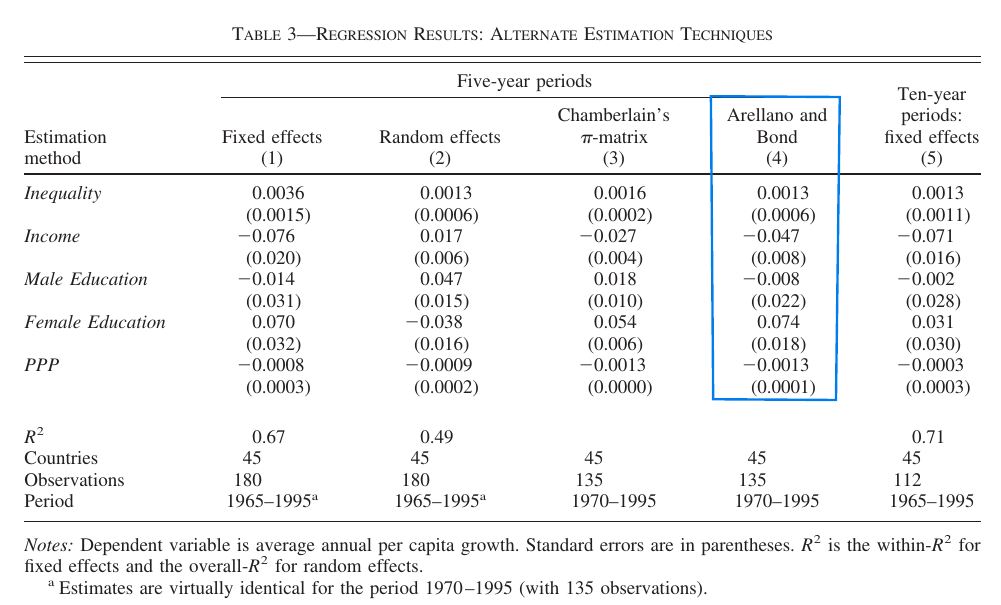
\includegraphics[scale=0.6]{forbes_tableau_3.png}
\caption{Tableau 3 de \cite{forbes}}
\label{tableau_3}
\end{center}
\end{figure}

\begin{figure}[h!]
\begin{center}
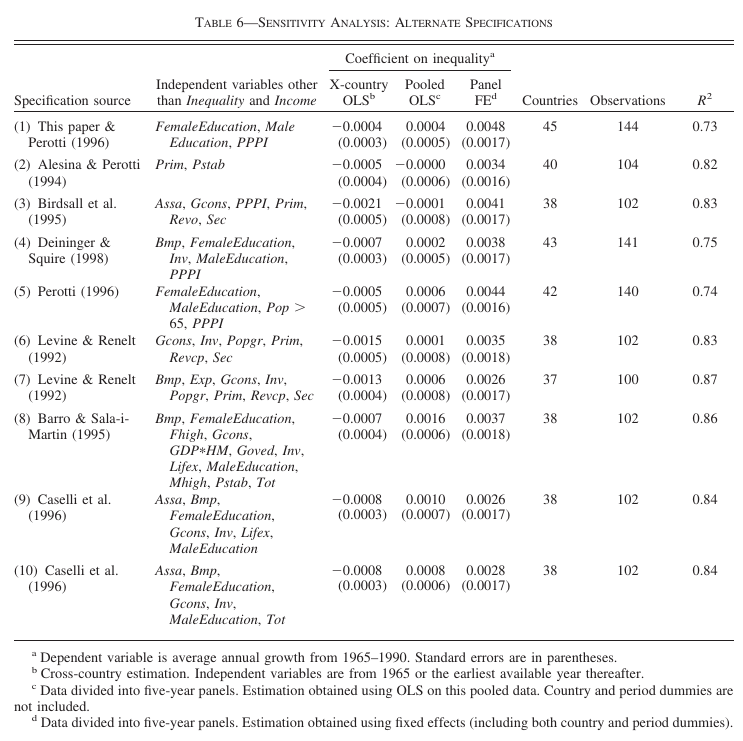
\includegraphics[scale=0.6]{forbes_tableau_6.png}
\caption{Tableau 6 de \cite{forbes}}
\label{tableau_6}
\end{center}
\end{figure}

Sur le tableau Figure \ref{tableau_6}, il est clair que l'un des facteurs déterminants du changement de signe du coefficient des inégalités est l'utilisation des variables \og dummy \fg~. L'auteure met également en avant sur le tableau 4 de son étude (non présenté ici) que le calcul de la moyenne sur une période de 5 années et non sur un période plus longue (comme dans l'étude de Perotti (1996) \cite{perotti} par exemple) peut en faire changer le signe. Nous attacherons moins d'importance à ce point car il est en apparence sans lien avec les remarques à venir. 


\section{Reproduction des calculs}

Intéressés par ces résultats, nous avons tenté de reproduire le plus fidèlement possible les traitements décrits. Nous avons donc téléchargé et arrangé les bases de données citées en référence en restant aussi proche que possible des indications de l'étude. L'ensemble des données, traitements et calculs (faits en python via jupyter notebook) sont disponibles en ligne \footnote{https://github.com/klemnnain/stage_M2/tree/master/forbes}. 

Malgré nos efforts, il a été impossible de  reproduire exactement la base de données utilisée dans l'étude. Certaines données, notamment celle de la worldbank ne sont plus disponibles dans l'état exact. Cependant nous somme parvenus à obtenir une base raisonnablement proche de la base de l'étude. La figure \ref{data_closeness} compare les valeurs moyennes, les écarts quadratiques, les valeurs minimales et maximales des deux bases de données.

\begin{figure}[h!]
\centering
\begin{subfigure}{0.55\textwidth}
  \centering
	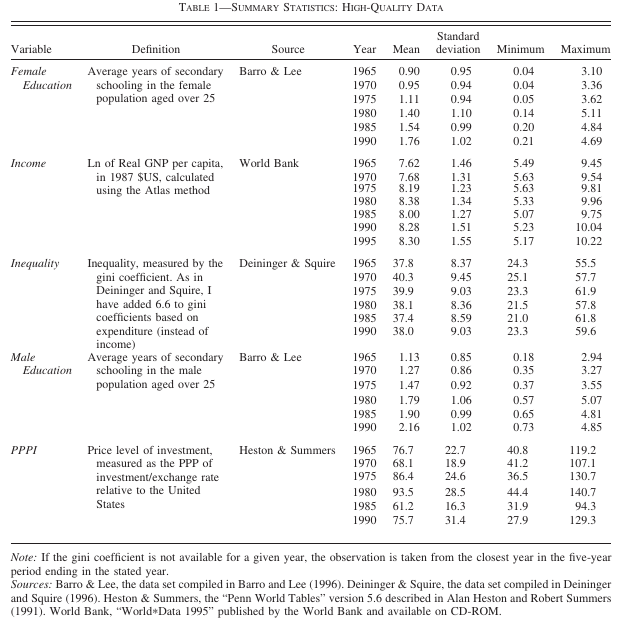
\includegraphics[scale=0.55]{forbes_tableau_1.png}
	\caption{Tableau 1 de \cite{forbes}}
	\label{tableau_1}
\end{subfigure}%
\begin{subfigure}{.45\textwidth}
  \centering
  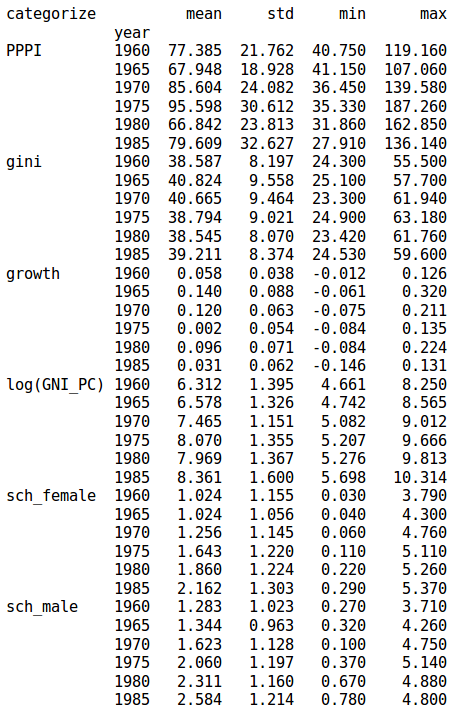
\includegraphics[width=.7\linewidth]{repro_data_resume.png}
  \caption{Recapitulatif du jeu de données reproduit}
  \label{data_resume}
\end{subfigure}
\caption{Comparaison de la base de Forbes avec notre base}
\label{data_closeness}
\end{figure}

Ne souhaitant pas s'attaquer au problème des variables retardées, nous nous sommes contentés de réaliser une régression linéaire ordinaire. C'est un algorithme que nous connaissons et que nous maîtrisons bien, à l'inverse de la méthode d'Arellano et Bond. Nous n'avons pas pris le temps d'investiguer en grand détail les différences fines entre les deux méthodes mais il nous semble raisonnable de dire que la critique formulée sur la régression linéaire s'applique aussi à la méthode plus complexe d'Arellano et Bond. Cette dernière méthode est introduite pour résoudre le problème de la variable retardée (la variable croissance contient la variable PIB) alors que notre critique se situe en amont dans la part de la variance absorbée par l'utilisation de \og dummies \fg~. La régression linéaire a par ailleurs l'avantage d'expliciter l'utilisation des ces \og dummies \fg{} alors qu'elle est cachée par le calcul des premières différences dans la méthode d'Arellano et Bond. 

En premier lieu, commençons par tracer sur la figure \ref{scatter_plot} la croissance en fonction de chacune des variables explicatives. Au vu de ces graphiques, force est de constater que les corrélations sont loin d'être évidentes.

\begin{figure}[h!]
\begin{center}
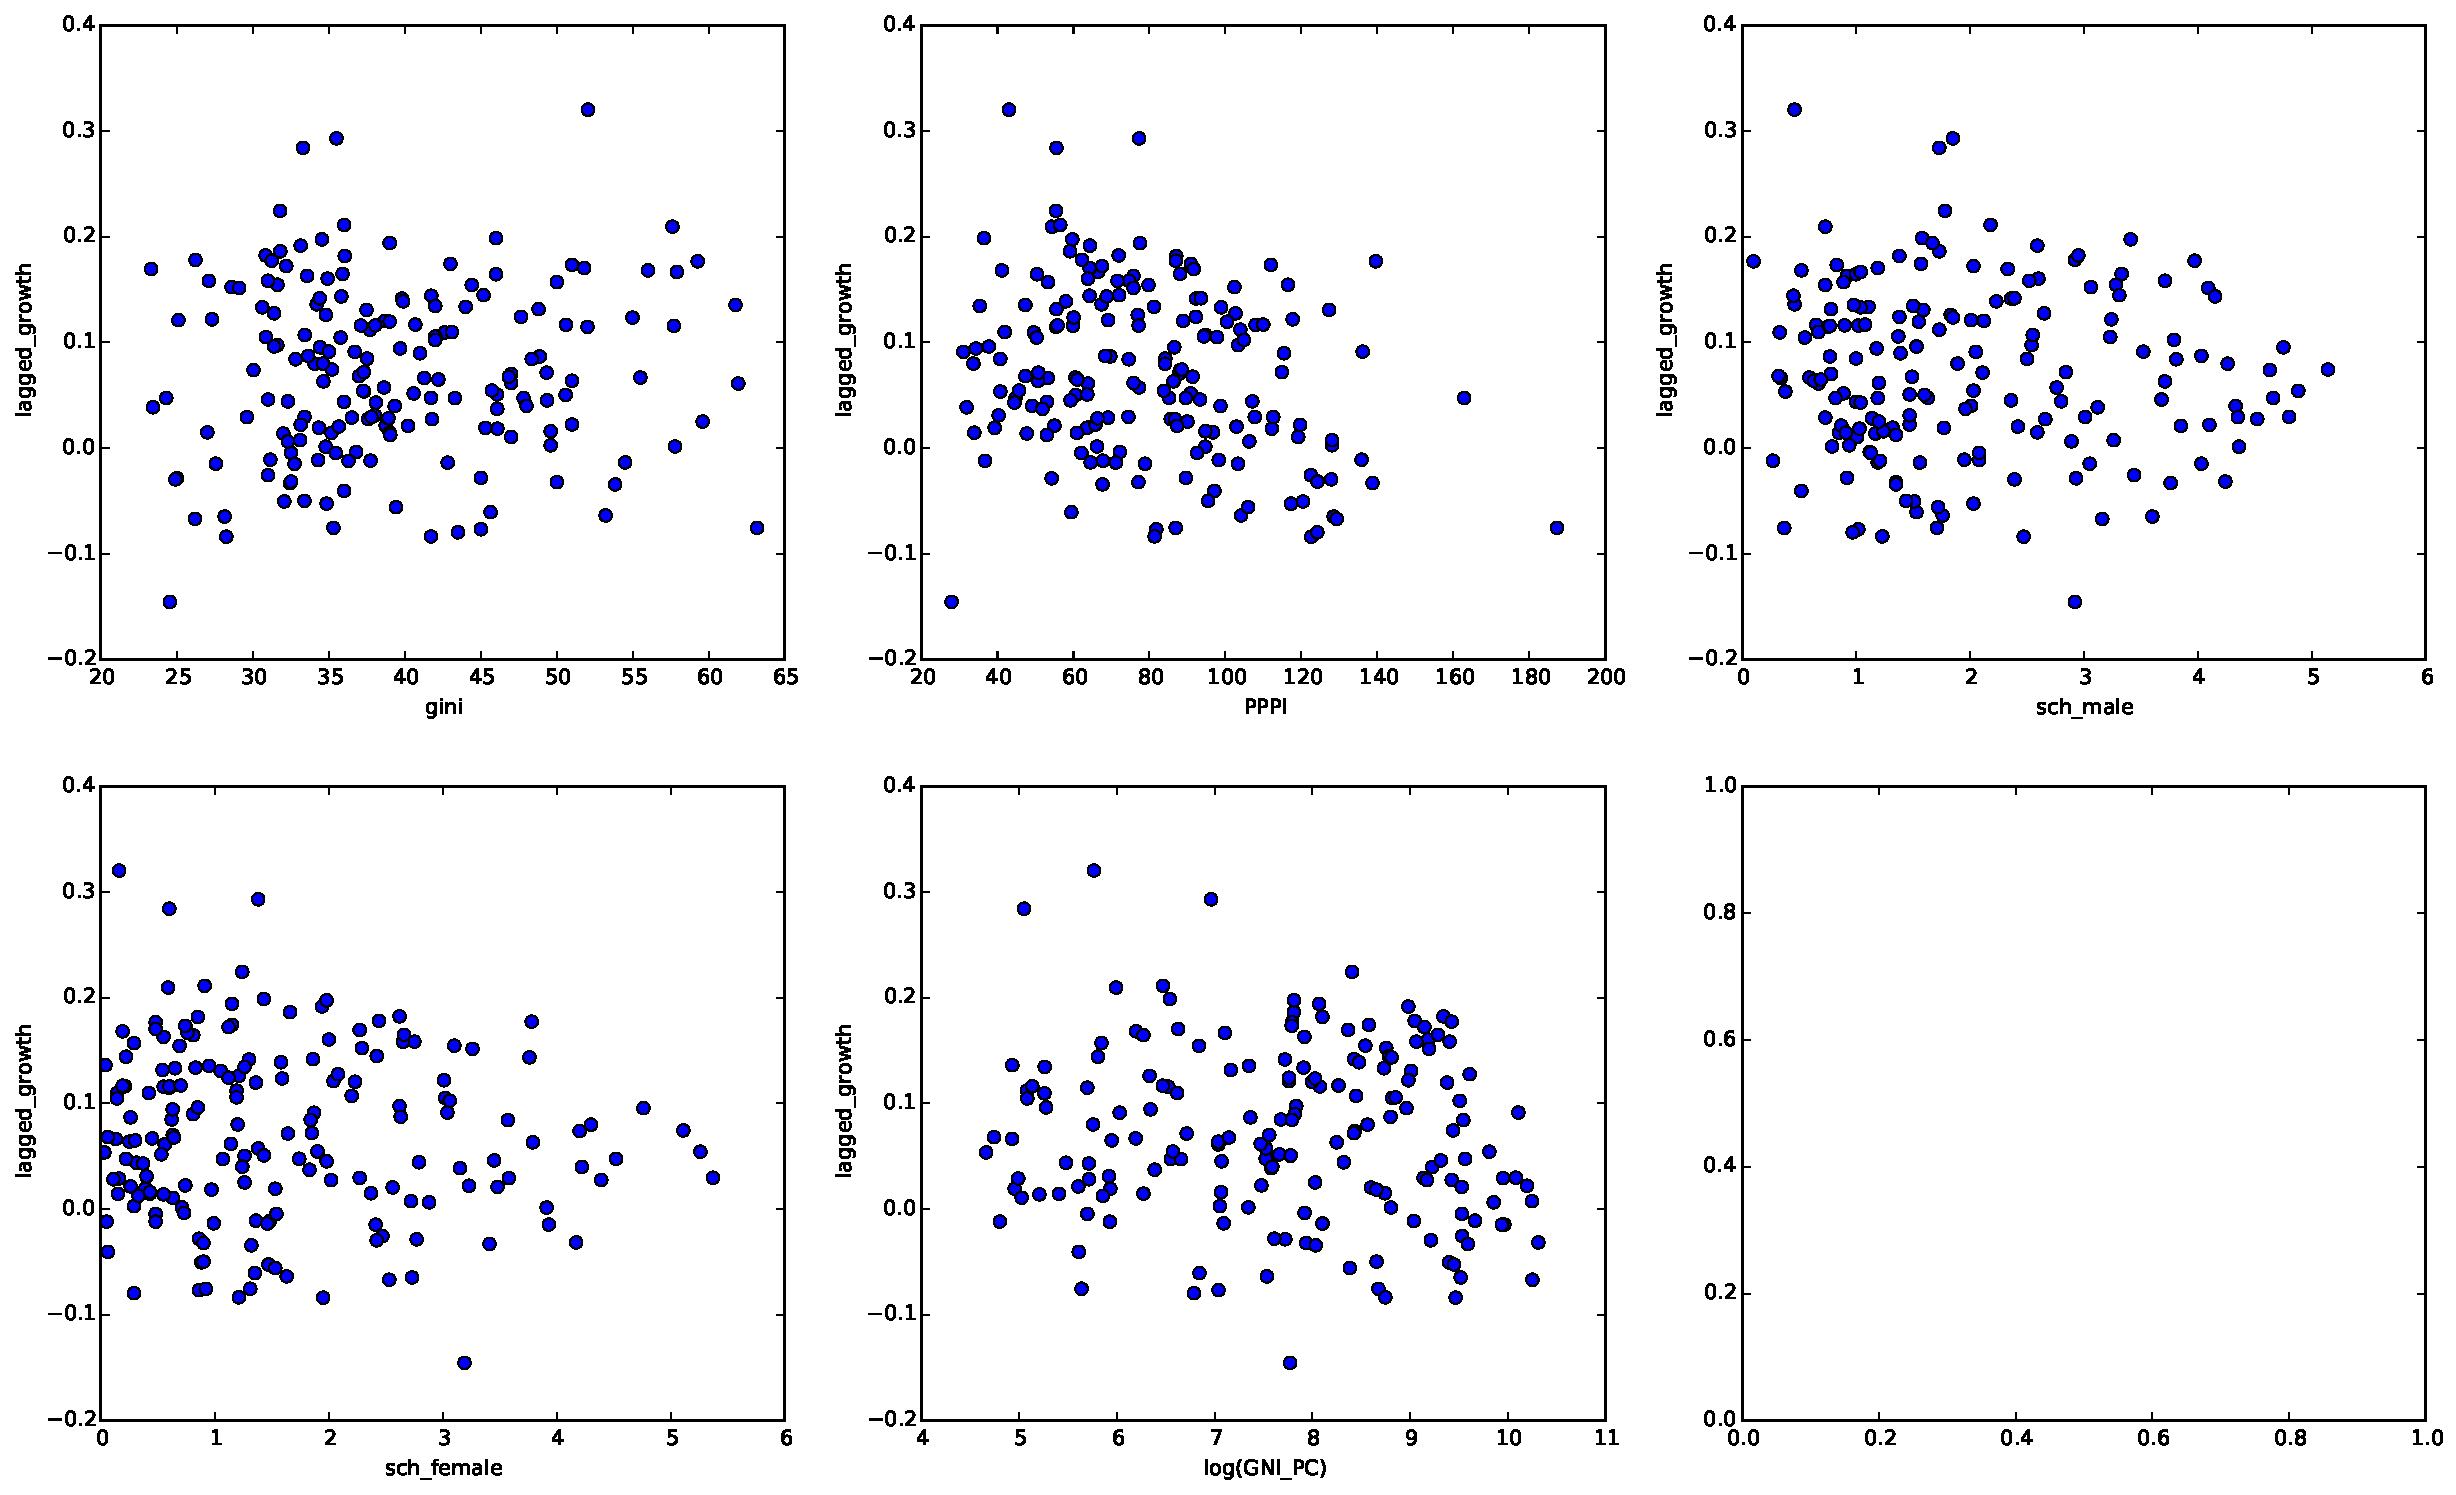
\includegraphics[scale=0.4]{scatter_plot_1.pdf}
\caption{Scatter plot de chaque variable explicative}
\label{scatter_plot}
\end{center}
\end{figure}

Nous ajoutons ensuite une \og dummy \fg~ pour chaque pays et une autre pour chaque période de temps. Nous ajoutons, par exemple, une variable "France" qui vaudra $1$ pour toutes les observations concernant la France et $0$ pour toutes les autres observations. On normalise ensuite les données en retranchant à chaque variable sa moyenne et en la divisant par sa variance. Grâce à cela on peut comparer directement l'influence des variables en regardant la valeur du coefficient de la régression linéaire.

Le tableau \ref{OLS_coef} donne les coefficients obtenus grâce à la régression linéaire ordinaire. Nous affichons deux résultats, ceux avec les données normalisées afin de pouvoir comparer l'importance relative des différents coefficients dans la régression linéaire et des coefficients non-normalisés afin de comparer avec les résultats de Forbes et d'avoir une idée de l'impact réel des différentes variables. On voit que les résultats pour les données non-normalisées sont assez proches des résultats de Forbes. La seule différence est un facteur 2 dans le coefficient devant les inégalités. Cette différence provient sans doute de petites différences dans les données, elle n'est pas problématique car elle va à l'encontre des résultats que nous cherchons à montrer : elle rend notre démonstration plus difficile. 


\begin{center}
\begin{tabular}{ l ll | ll }
 & Normalized coef & Normalized std & Coefficients & std\\
gini      &  0,6495  &  0,188  &  0,0060  &  0,0018  \\ 
PPPI       &  -0,4525  &  0,126  &  -0,0014  &  0,0004  \\ 
sch_male    &    0,9552  &  0,568  &  0,0637  &  0,0381  \\ 
sch_female   &   0,1607  &  0,588  &  0,0197  &  0,0383  \\ 
log(GNI_PC)  & -1,4715 &  0,352  &  -0,0820  &  0,0191 \\
R-squared:      &                 0.725 \\
\label{OLS_coef}
\end{tabular}
\captionof{table}{Coefficient de la régression linéaire simple}
\end{center}


Les points bleus de la figure \ref{OLS_graph} représentent les données de croissance à prédire et la courbe rouge en pointillée est la prédiction que nous sommes parvenus à faire avec les variables explicatives. La prédiction semble performante et la courbe rouge est proche des données, signe que le nombre de variables explicatives est suffisant. Environ $3/4$ de la variance est expliquée. 

\begin{figure}
  \centering
  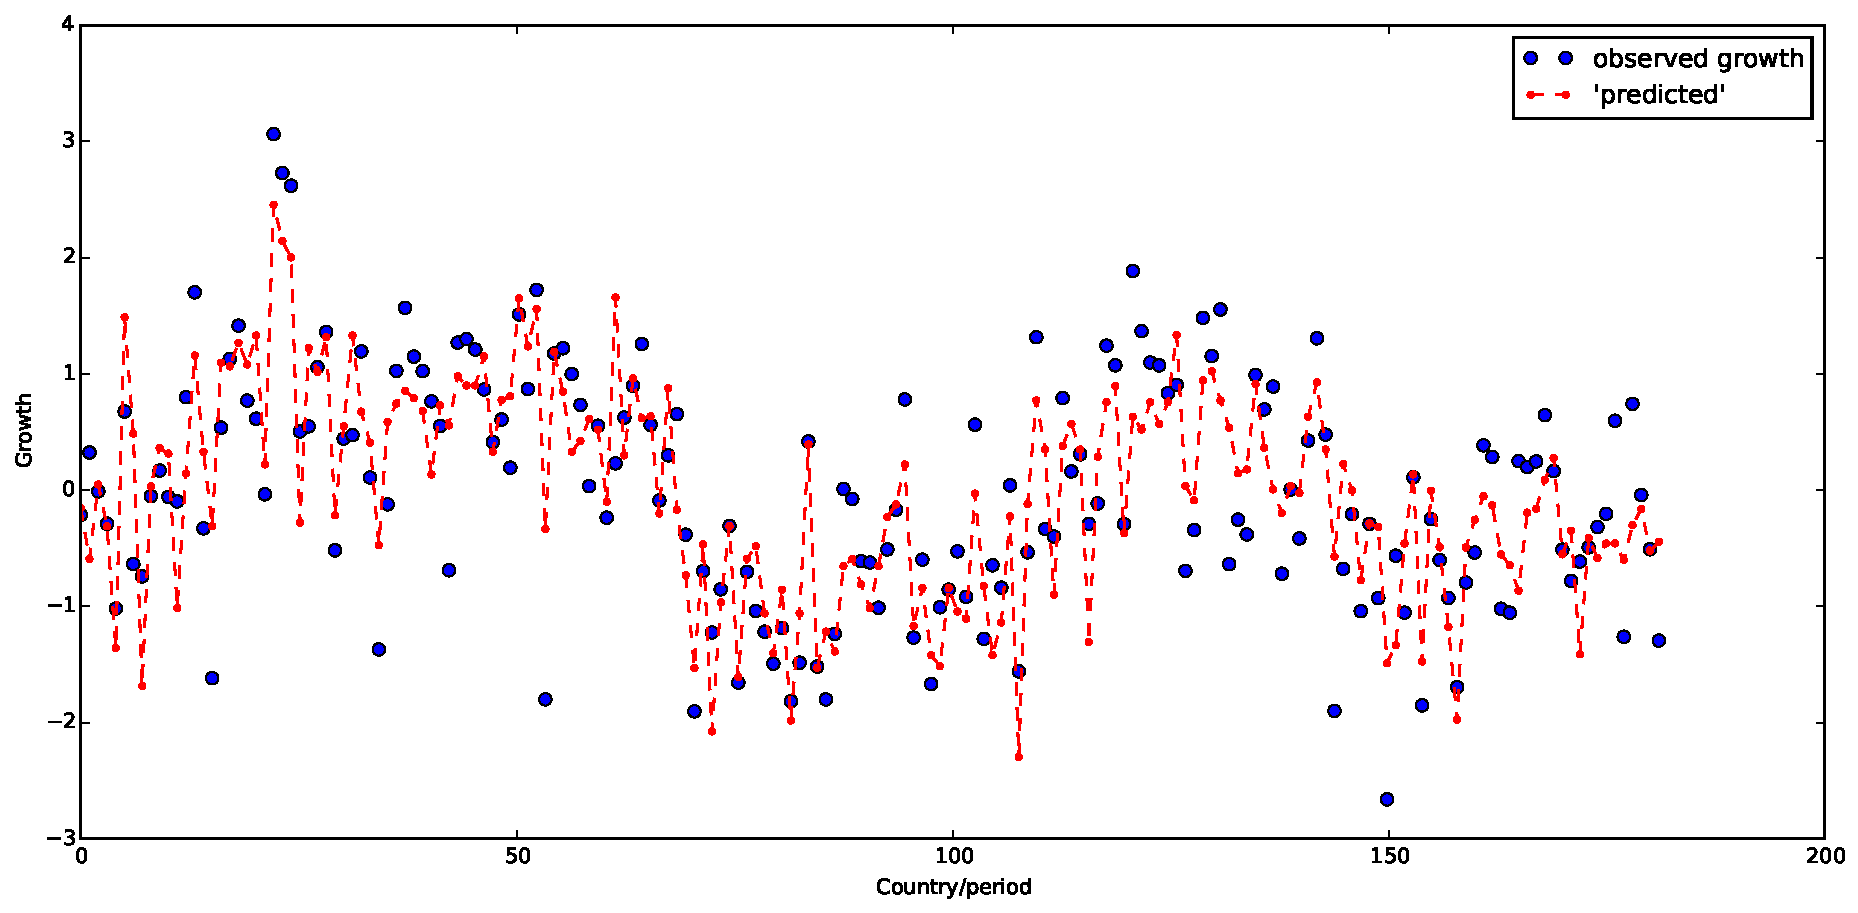
\includegraphics[width=1.\linewidth]{OLS_results.pdf}
\caption{Résultat de la régression linéaire ordinaire}
\label{OLS_graph}
\end{figure}


\section{Une répartition inégale de la variance ?}

La reproduction des résultats précédents nous a amené à nous interroger sur la part explicative de chaque variable dans la régression précédente. Une fois que l'on s'est focalisé sur les variations autour de la valeur moyenne de chaque pays, que reste-t-il à prédire et quelle part est réellement prédite par les variables ? Une première approche très simple pour aborder ce problème est de réaliser la régression linéaire précédente en deux temps. Tout d'abord nous allons effectuer la régression en utilisant uniquement les variables \og dummy \fg~ ensuite nous effectuerons une régression avec les variables restantes en prenant le résidu de la régression précédente comme variable à prédire. 

\begin{center}
\begin{tabular}{ l c r }
Explained variance share : first step &  54.7 \% \\
Explained variance share : second step &  2.8 \% \\
gini     &    0.03 \\
PPPI      &  -0.18 \\
sch_male   & -0.03 \\
sch_female &  0.05 \\
log(GNI_PC) &  0.03 \\
\label{OLS_coef}
\end{tabular}
\captionof{table}{Coefficient de la régression linéaire ordinaire}
\end{center}


\begin{figure}
  \centering
  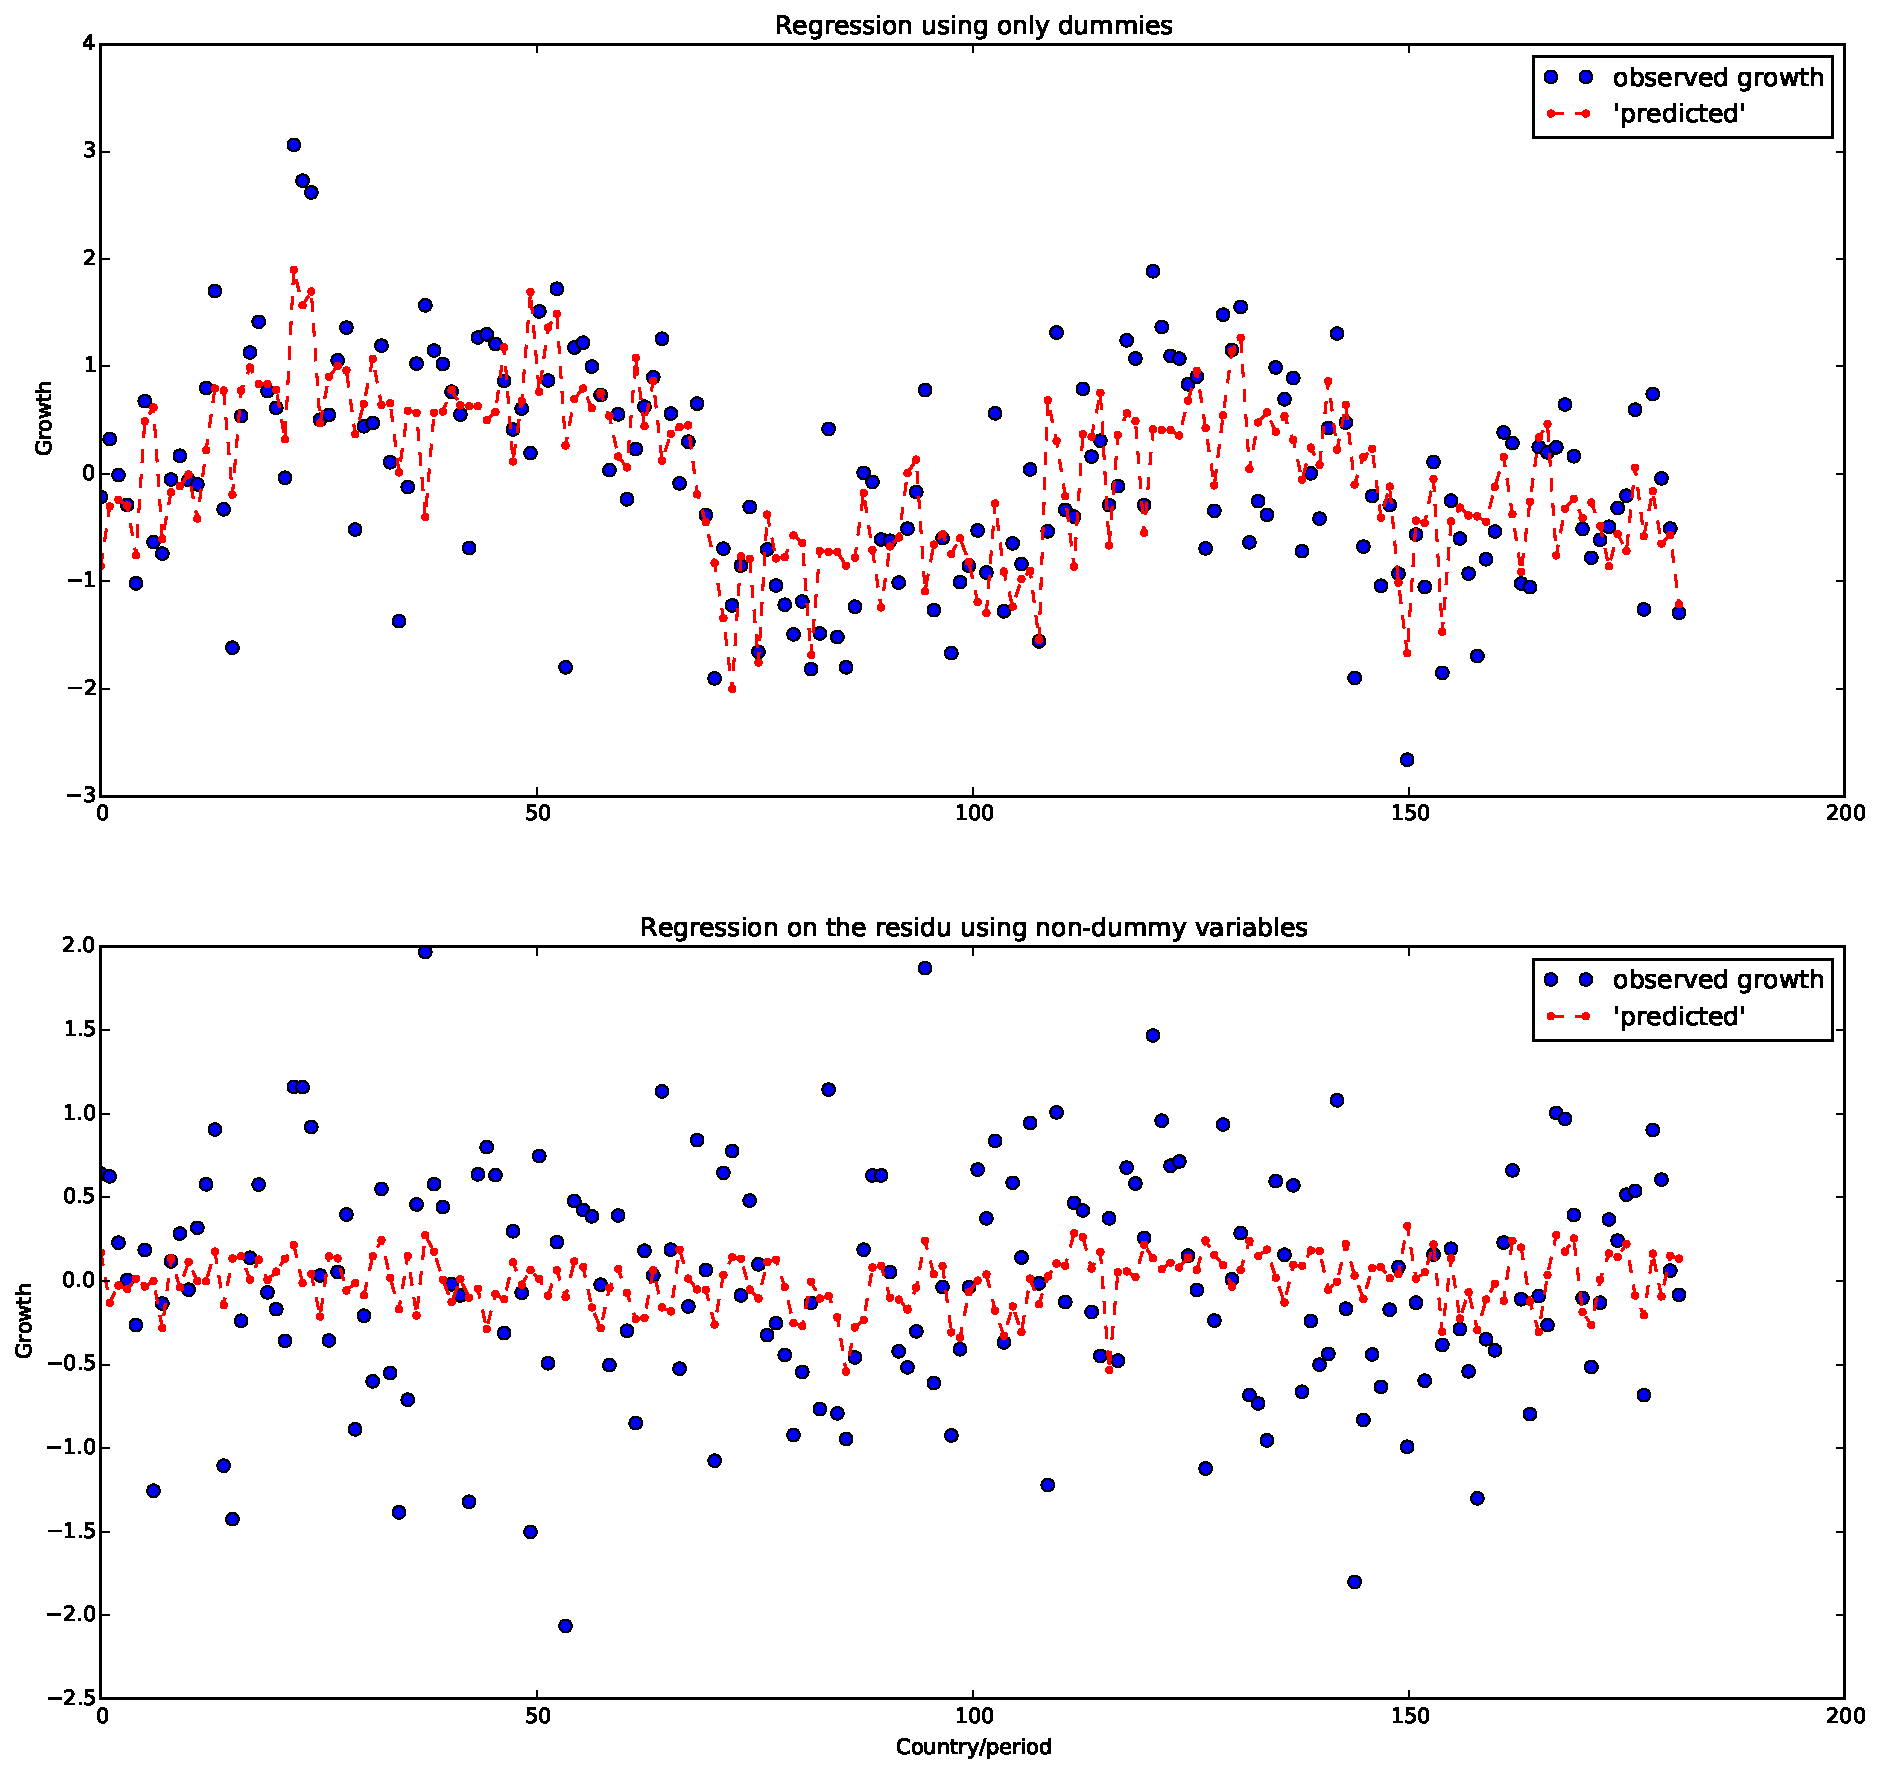
\includegraphics[width=1.\linewidth]{two_steps_OLS.pdf}
\caption{Résultat de la régression linéaire ordinaire en deux étapes}
\label{2s_OLS_graph}
\end{figure}

On peut voir sur la figure \ref{2s_OLS_graph} que lorsque la régression est effectuée avec les variables \og dummy \fg~ en premières, une part très importante de la variance est absorbée par cette étape. Qui plus est, le résidu de cette première régression semble très difficile à prédire puisqu'on voit que la part de la variance expliquée lors de la deuxième étape de la régression est quasiment nulle. Il est alors légitime de questionner l'utilisation de ces \og dummies \fg{} avec si peu de données. 

Il semble clair qu'avec nettement plus de données le problème ne se poserait pas. S'il on avait 300 points par pays, on pourrait \textit{a priori} prédire beaucoup moins de variance avec la simple valeur moyenne. Il pourrait donc s'agir d'un problème de sur-optimisation des coefficients. Pour vérifier cette hypothèse, nous utiliserons une procédure de validation croisée. La validation croisée donne une image réaliste du pouvoir prédictif d'un modèle. 

Les modèles économiques empiriques sont basés sur des données historiques et ont pour but de guider les politiques économiques futures. En d'autres termes, les modèles doivent s'entraîner (\textit{i.e.} ajuster leurs coefficients) sur certaines données et tester leurs précisions sur d'autres données que le modèle n'a jamais vu et qui représenterait le futur, l'inconnu. La validation croisée permet de reproduite artificiellement ce schéma d'apprentissage à partir d'un seul jeu de données (voir \cite{hastie} pour plus d'informations). 

Pour ce faire, nous avons divisé le jeu de données en 5 parties de tailles égales composées d'observations tirées aléatoirement dans le jeu de données. Nous avons ensuite entraîné nos modèles sur $4 / 5$ des données (\textit{i.e.} calculé les coefficients) et testé leurs validités sur le $1 / 5$ restant en calculant l'écart des prédictions aux données. Cela nous permet de connaître la capacité d'un modèle à produire une prédiction sur des données qu'il n'a jamais vu. Cette méthode nous permet de comparer deux modèles, le premier est la régression linéaire ordinaire le deuxième est un modèle de Lasso. Ce dernier est un modèle de régression linéaire ordinaire avec un terme de pénalisation des coefficients qui autorise à écarter certaines variables du modèle prédictif lorsqu'elles participent seulement à la sur-optimisation des des coefficients aux données et qu'elles n'apportent rien à la prédiction sur les données nouvelles (voir \cite{hastie_lasso} pour plus de détails). $1 / 5$ des données représentant peu de points, il se peut que le cinquième choisi ne soit pas distribué de manière représentative du jeu complet. Pour palier à ce problème nous avons effectué la procédure un grand nombre de fois (2000 * 5) et avons moyenné les résultats obtenus. 


Les résultats de ce test sont très instructifs. En premier lieu, on peut constater sur la figure \ref{OLS_Lasso_graph} que le modèle Lasso a diminué la valeur des coefficients de la régression, on peut voir cela à l'apparent lissage de la courbe. En regardant les résultats sur la table \ref{OLS_Lasso_coef}, on peut voir que la part de la variance expliquée est nettement plus faible pour la validation croisée ce qui est normal puisque le modèle doit maintenant prédire une valeur sur des données qu'il n'a jamais vu ce qui est plus difficile mais aussi plus réaliste. Deuxièmement, ce test valide bien l'hypothèse de la sur-optimisation des coefficients. En effet, le modèle de Lasso, dont les coefficients ont été artificiellement réduits par pénalisation, obtient en moyenne, de meilleurs résultats (cf. tableau \ref{OLS_Lasso_coef}). 


\begin{center}
\begin{tabular}{ l c r }
 & mean & std \\
Explained variance share : OLS &  0.312676319641  & 0.120855814149 \\
Explained variance share : Lasso &  0.264664473665 & 0.237392947754 \\
\label{OLS_Lasso_coef}
\end{tabular}
\captionof{table}{Résultats du test de sur-optimisation}
\end{center}

\begin{figure}
  \centering
  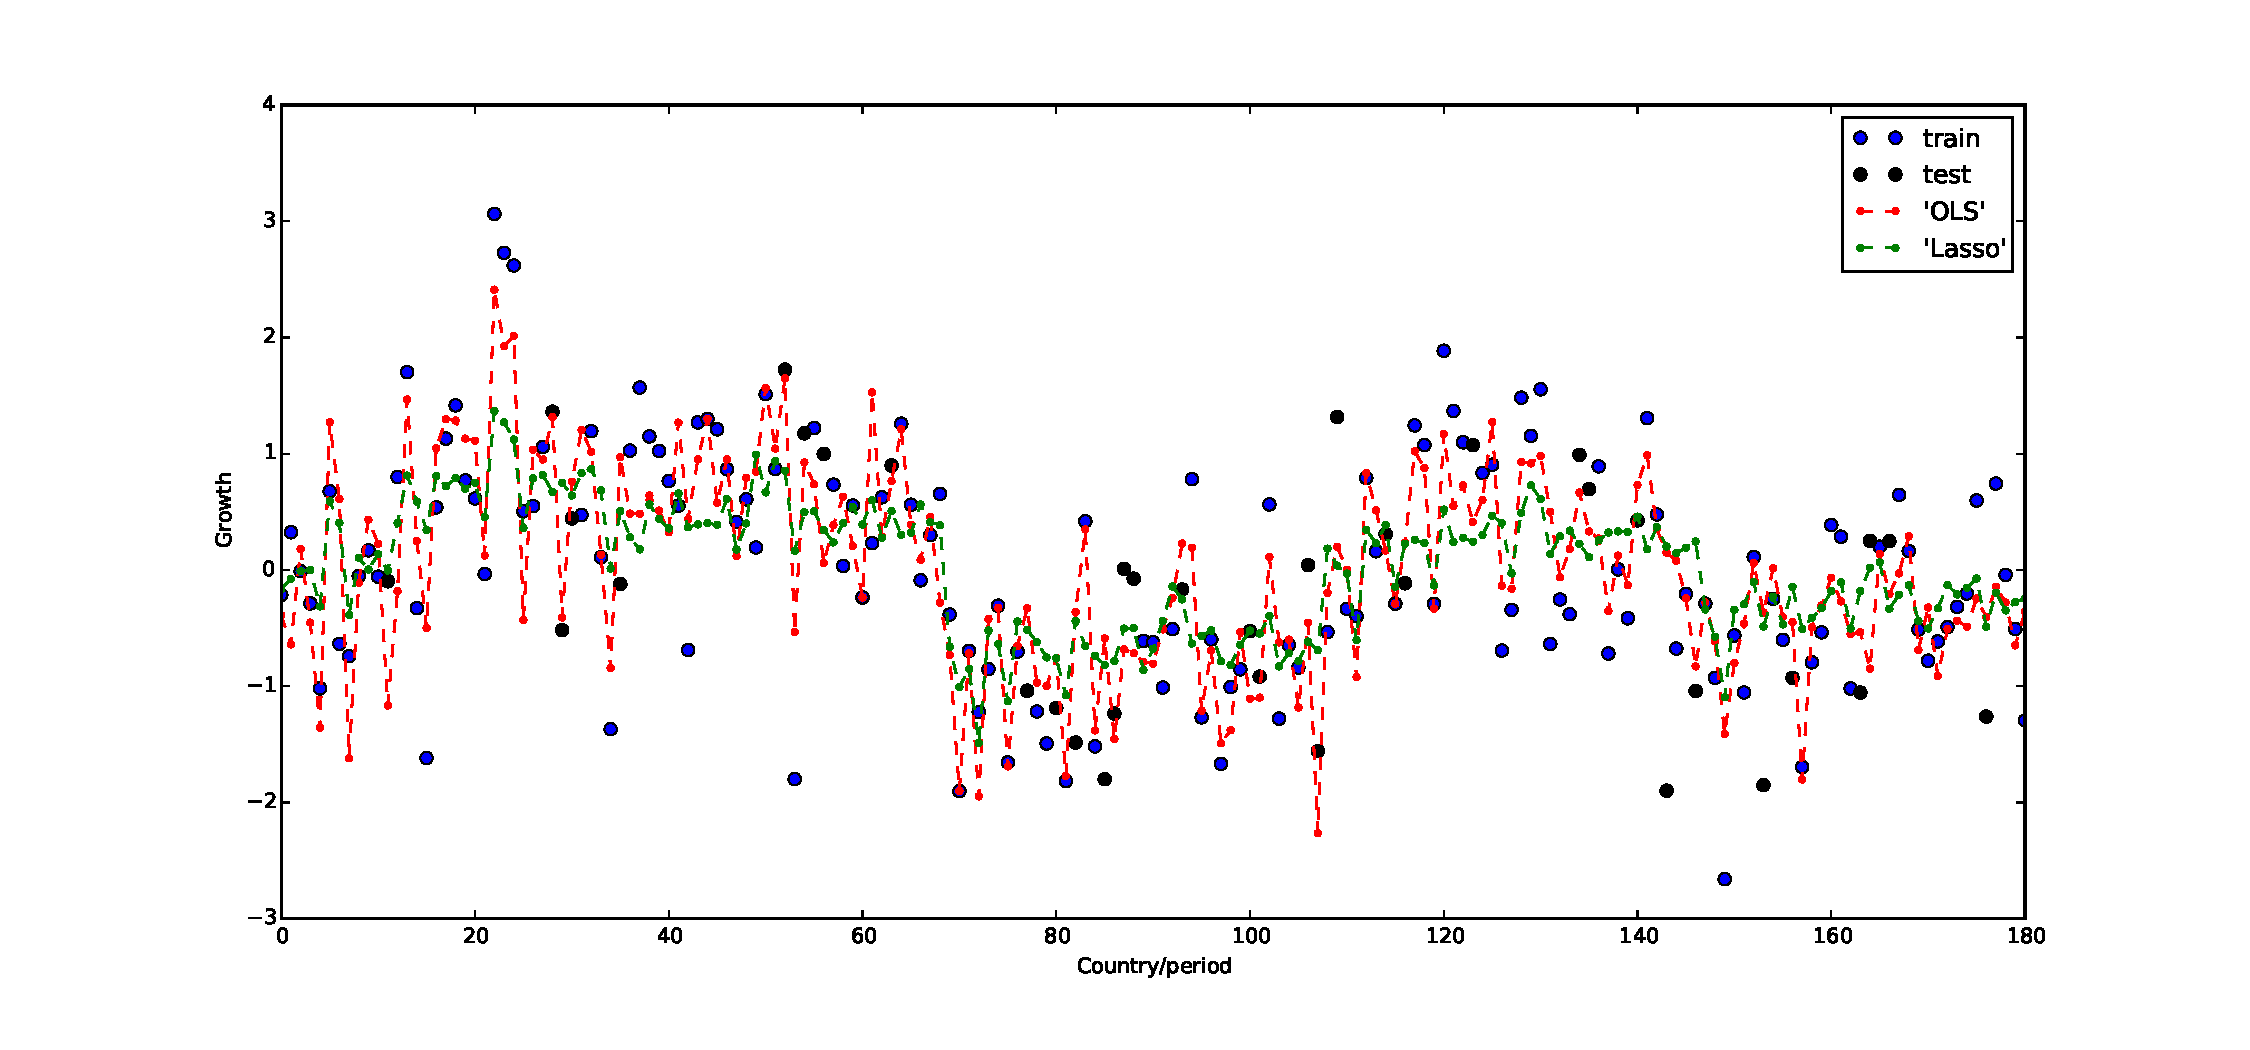
\includegraphics[width=1.\linewidth]{OLS_Lasso.pdf}
\caption{Comparaison de la prédiction par le Lasso et par le modèle linéaire}
\label{OLS_Lasso_graph}
\end{figure}

Le résultat le plus instructif de cette expérience vient de l'étude des coefficients de la régression de Lasso. Ces coefficients peuvent être interprétés exactement de la même manière que les coefficients d'une régression linéaire. On peut voir sur le tableau 4. que seule la variable $PPPI$ a un coefficient non-négligeable et que le reste de la prédiction est en fait assurée par les \og dummies \fg. On voit en particulier que le coefficient pour la variable $gini$ est de l'ordre de $10^{-6}$ en moyenne sur toutes les simulations. \textbf{Grâce à ces résultats on vient de prouver que la prédiction la plus précise que nous puissions faire de la croissance à partir de ces données ne prend pas en compte le coefficient de Gin !}


\begin{center}
\begin{tabular}{ ll | ll | ll }
1975&-3.16e-01&     CIV& -1.54e-02&     MYS&  3.69e-05\\ 
1985&-1.99e-01&     TTO& -1.10e-02&     GBR&  2.84e-05\\ 
PPPI&-1.64e-01&     ITA&  8.25e-03&     BRA&  2.41e-05\\ 
1965& 1.44e-01&     log(GNI_PC)&    6.79e-03&   USA& -1.80e-05\\ 
1970& 1.33e-01&     NOR&  6.21e-03&     TUR& -6.02e-06\\ 
BGR& -1.16e-01&     FIN&  5.03e-03&     1980& 3.88e-06\\ 
JPN&  9.97e-02&     DEU&  4.45e-03&     \hl{gini}&\hl{-3.88e-06}\\ 
KOR&  7.26e-02&     PRT& -4.14e-03&     DNK&  1.18e-06\\ 
IND& -5.62e-02&     sch_male&     4.02e-03&     CAN& -8.98e-08\\ 
IRN&  5.61e-02&     GAB&  3.54e-03&     AUS&  0.00e+00\\ 
CHL& -5.47e-02&     FRA&  2.44e-03&     sch_female&     0.00e+00\\
BGD& -4.86e-02&     NLD&  9.42e-04&     COL&  0.00e+00\\ 
VEN& -4.58e-02&     ESP&  7.38e-04&     TUN&  0.00e+00\\ 
HKG&  4.17e-02&     BEL& -2.40e-04&     CHN&  0.00e+00\\ 
SGP&  3.99e-02&     PHL& -2.30e-04&     GRC&  0.00e+00\\ 
DOM& -3.65e-02&     IDN& -9.85e-05&     PER&  0.00e+00\\ 
1960&-3.10e-02&     SWE&  8.51e-05&     CRI&  0.00e+00\\ 
PAK& -2.83e-02&     THA&  7.56e-05&     NZL&  0.00e+00\\ 
LKA& -2.40e-02&     MEX& -3.70e-05&     IRL&  0.00e+00\\
\label{lasso}
\end{tabular}
\captionof{table}{Coefficients de la régression de Lasso. Ces coefficients sont la moyenne des coefficients sur 2000 * 5 simulations. }
\end{center}

Cette nouvelle approche met en doute la méthode de Forbes et la possibilité d'ajouter des \og dummy \fg~variables sans précautions particulières. La même méthode a été reprise dans d'autres études \cite{ostry}, \cite{OCDE}. Nous ne pouvons aucunement remettre en doute la validité de ces études à partir des simples remarques faites pour Forbes car les données utilisées sont très différente (le nombre de points par pays est notamment beaucoup plus élevé). Cependant, si les remarques faites dans cette note sont pertinentes, alors il serait légitime d'appliquer la même méthode d'analyse à ces études pour tester la validité des mêmes hypothèses dans les autres études. 

\newpage

\noindent
\textbf{Conclusion :}\\

Cette note n'a pas vocation à remettre en question les résultats produits par l'étude de Forbes mais plutôt de formaliser nos interrogations sur la méthode utilisée. Même si nos intuitions se révèlent pertinentes, cette note ne constitue pas une preuve de la fausseté des résultats de Forbes. De nombreux points pouvant avoir une influence cruciale sur les résultats restent non-traités dans cette note. Premièrement, une preuve sérieuse doit s'assurer que les données utilisées sont rigoureusement les mêmes que celles de Forbes. Même s'il nous semble que le jeu que nous avons réussi à créer est de bonne qualité qu'une étude se doit d'être robuste à quelques différences minimes dans les données, il serait plus rigoureux d'obtenir (par exemple en demandant à l'auteure) le jeu de données utilisé pour l'étude. Le deuxième point limite de l'étude est l'utilisation de la régression linéaire au lieu de la méthode d'Arellano et Bond. Si nos intuitions se révèlent exactes, l'étape suivante serait d'appliquer la même procédure de validation croisée pour tester la méthode Arellano et Bond et particulièrement la robustesse du signe du coefficient de gini. Enfin cette étude, réalisée en marge d'un stage de M2, a été faite en peu de temps (d'où notre préférence pour des algorithme connus) et sans concertation avec l'auteure de l'étude, la validation des nos hypothèses pourrait commencer par un contact avec cette dernière pour avoir son avis sur nos remarques. 

\begin{thebibliography}{99}
\bibitem{forbes}
	Forbes, Kristin J. 2000. \emph{A Reassessment of the Relationship between Inequality and Growth.} American Economic Review, 90(4): 869-887.

\bibitem{banerjee}
Banerjee, Abhijit V. and Duflo, Esther, \emph{Inequality And Growth: What Can The Data Say?} (June 2000). MIT Dept. of Economics Working Paper No. 00-09. Available at SSRN: http://ssrn.com/abstract=232731 or http://dx.doi.org/10.2139/ssrn.232731 

\bibitem{perotti}
Perotti, Roberto. \emph{Growth, Income Distribution, and Democracy: What the Data Say}. Journal of Economic Growth 1.2 (1996): 149–187. Web...

\bibitem{ostry}
Jonathan D. Ostry, Andrew Berg, and Charalambos G. Tsangarides, \emph{Redistribution, Inequality, and Growth}. IMF Staff Discussion Note. February 2014. 

\bibitem{OCDE}
OECD.  (2015), In It Together: Why Less Inequality Benefits All, OECD Publishing, Paris.
DOI: http://dx.doi.org/10.1787/9789264235120-en

\bibitem{hastie}
Trevor Hastie, Robert Tibshirani, Jerome Friedman \textit{The Elements of Statistical Learning: Data Mining, Inference, and Prediction.} Second Edition February 2009, p. 241 - 245, disponible en ligne : http://statweb.stanford.edu/~tibs/ElemStatLearn/

\bibitem{hastie_lasso}
Trevor Hastie, Robert Tibshirani, Jerome Friedman \textit{The Elements of Statistical Learning: Data Mining, Inference, and Prediction.} Second Edition February 2009, p. 68 - 69, disponible en ligne : http://statweb.stanford.edu/~tibs/ElemStatLearn/

\end{thebibliography}

\end{document}
